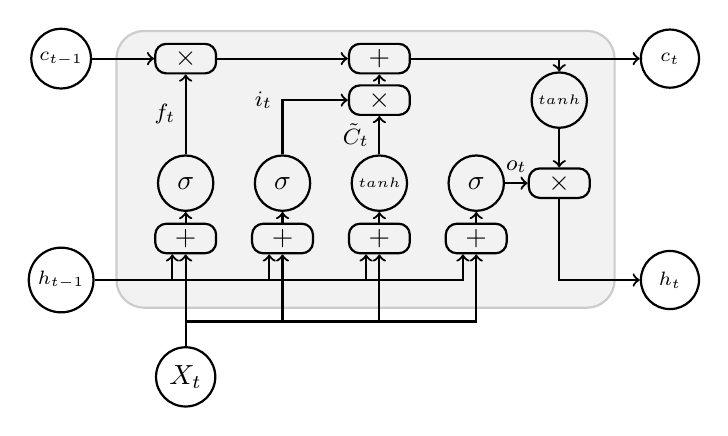
\begin{tikzpicture}

		\tikzstyle{operation} = [rectangle, thick,draw,align=center, minimum width=2.2em, minimum height=.5em,inner sep=2pt,rounded corners=4 ]
		
		\tikzstyle{links} = [->, thick]
		
		\tikzstyle{values} = [circle, draw, thick, inner sep = 2,minimum size=2.1em]
		
		\tikzstyle{functions} = [draw, circle, thick, inner sep=1, minimum size=20]
		
		\draw[rounded corners=10,black!20!white, thick, fill=black!5!white ] (0,0) rectangle (18em,-10em);
		
		\node[operation] at (2.5em, -7.5em) (addition1) {$+$};
		\node[operation] at (6em, -7.5em) (addition2) {$+$};
		\node[operation] at (9.5em, -7.5em) (addition3) {$+$};
		\node[operation] at (13em, -7.5em) (addition4) {$+$};
		
		
		\node[functions] at (2.5em, -5.5em) (sigma1) {$\sigma$};
		\node[functions] at (6em, -5.5em) (sigma2) {$\sigma$};
		\node[functions] at (9.5em, -5.5em) (tanh1) {\tiny $tanh$};
		\node[functions] at (13em, -5.5em) (sigma3) {$\sigma$};
		
		
		\node[operation] at (9.5em, -2.5em) (times1) {$\times$};
		\node[operation] at (9.5em, -1em) (addition5) {$+$};
		
		\node[operation] at (16em, -5.5em) (times2) {$\times$};
		\node[functions] at (16em, -2.5em) (tanh2) {\tiny $tanh$};
		
		\node[operation] at (2.5em, -1em) (times3) {$\times$}; 
		
		\node[circle, draw, thick, inner sep = 2.5] at (2.5em, -12.5em) (input) {$X_t$};
		
		
		
	%	\node[circle, draw, thick, inner sep = 2.5, left = 2.5em of times3] (previouscellstate) {\scriptsize $c_{t-1}$} ;
		
		\node[values] at (-2em,-1em) (previouscellstate) {\scriptsize $c_{t-1}$} ;
		
		\node[values] at (-2em,-9em) (previoushiddenstate) {\scriptsize $h_{t-1}$} ;
		
		\node[values] at (20em,-9em) (nexthiddenstate) {\scriptsize $h_{t}$} ;
		
		\node[values] at (20em, -1em) (nextcellstate) {\scriptsize $c_{t}$} ;
		
		\draw[links] (previouscellstate) -- (times3);
		\draw[links] (addition5) -- (nextcellstate);
		
		\draw[links] (input) -- (addition1);
		\draw[links] (input) |- ++(3em,2em) -| (addition2);
		\draw[links] (input) |- ++(5em,2em) -| (addition3);
		\draw[links] (input) |- ++(7em,2em) -| (addition4);
		
		\draw[links] (previoushiddenstate) -|  (addition1.230);
		\draw[links] (previoushiddenstate) -|  (addition2.230);
		\draw[links] (previoushiddenstate) -|  (addition3.230);
		\draw[links] (previoushiddenstate) -|  (addition4.230);
		
		\draw[links] (times2) |- (nexthiddenstate);
		
		\draw[links] (addition1) -- (sigma1);
		\draw[links] (addition2) -- (sigma2);
		\draw[links] (addition3) -- (tanh1);
		\draw[links] (addition4) -- (sigma3);
		
		\draw[links] (tanh1) -- node[left] {\footnotesize $\tilde{C}_t$} (times1);
		\draw[links] (times1) -- (addition5);
		\draw[links] (sigma2)    |-  node[left] {\footnotesize $i_t$} (times1) ;
		
		\draw[links]  (sigma1)  -- node[left] {\footnotesize $f_t$} (times3);
		
		\draw[links] (times3) -- (addition5);
		\draw[links] (addition5) -| (tanh2);
		\draw[links] (tanh2) -- (times2);		
		\draw[links] (sigma3) -- node[above] {\footnotesize $o_t$} (times2);
	\end{tikzpicture}